\documentclass[12pt]{article}
\usepackage{f1000_styles}
\usepackage[numbers]{natbib}
\usepackage{hyperref,url,setspace}

\usepackage{booktabs}

\onehalfspacing

\begin{document}
\title{CODECHECK: An open-science initiative to facilitate sharing of
  computer programs and results presented in scientific publications.}
\author[1,$\ast$]{Daniel N\"{u}st}
\author[2,$\ast$]{Stephen J Eglen}
\affil[1]{\url{https://orcid.org/0000-0002-0024-5046}}
\affil[2]{\url{https://orcid.org/0000-0001-8607-8025}}
\affil[$\ast$]{Contributed equally}
\maketitle
\begin{abstract}
\ldots{}
\end{abstract}

\section*{TODO}\label{todo}

\begin{itemize}
\item Check with Giuliano re: ``code works''. Write to Naomi.
\end{itemize}

\section*{Introduction}\label{introduction}

Many areas of scientific research now use computation to either simulate
or analyse their data. These computations are increasingly complex, and
difficult to explain coherently in a paper. (MARWICK). To complement the
traditional route of sharing research by writing papers, there is a
growing trend/demand to share the underlying artifacts, notably code and
datasets, so that others can inspect, reproduce or expand that work
(Figure 1). Some of the earliest proponents were Buckheit and Donoho
(1995) who commented ``advert is scholarship for the paper''. (get
correct quote).

So, assuming that researchers begin to share more artifacts, how might
they be examined to test that they do what they claim? For example,
most scientific journals now require a data sharing statement that
outlines what data the authors have (or will) share. The
implementation status of this varies considerably according to the
journal. At one of the spectrum, there are specialist journals that
have been created to accept ``data papers'' (e.g.~\emph{Scientific
  Data}, \textit{Geoscience Data Journal}\ldots{} NAME COUPLE OF
OTHERS). These journals have established rigorous procedures by which
the data is validated according to standards in each field. At the
other end of the spectrum, we still witness today the infamous
statement ``Data available upon reasonable request'' whereby authors,
well-intentioned, often cannot provide the data when readers ask for
it.  (ANDREW H: any references to sum up poor/evolving state of data
sharing; Vines et al 2014).

Given that there are no clear standards yet for sharing data, what hope
might there be for sharing computer programs? Our anectodal experiences
on this matter suggest that often a variety of reasons are given for why
their code cannot be shared, e.g.~``there is no documentation / I do not
want to maintain it / I do not want to give away my code to my
competitors''. Our view, rooted in open science princples, is that
wherever possible sharing code is good for the community, as outlined
ten years ago \cite{Barnes2010-iv}. Having the code freely available, and
suitably archived, provides a valuable resource for others to learn
from, even when it doesn't run or if there is no documentation. However,
with a little effort, we believe that if someone independent can run/use
the code, this is worth documenting as early as possible. With this in
mind, we have developed a set of PRINCIPLES and an example workflow that
provides what he hope is a pragmatic way of checking that code works. We
call this system CODECHECK as outlined next.

\begin{figure}
  \centering
  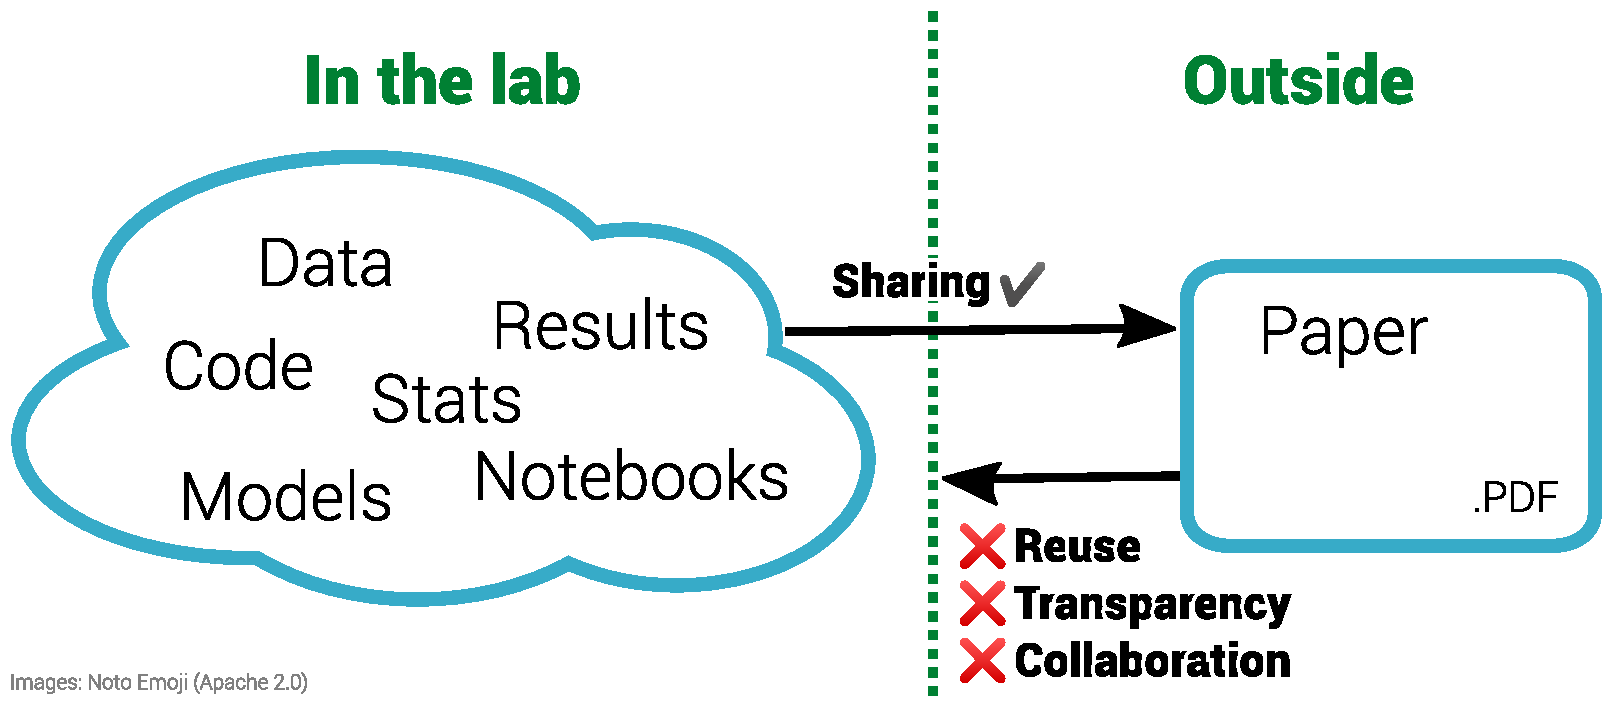
\includegraphics[width=\textwidth]{figs/rr.pdf}
  \caption{The inverse problem in reproducible research.  The left
  half of the diagram shows the diverse range of materials used
  internally within a laboratory.  These materials are often then
  condensed into a paper for sharing with the outside world via the
  research paper, a static PDF document.  Working backwards from the
  PDF to the underlying materials is impossible.  By sharing the
  materials on the left, others outside the lab are able to reproduce
  or build on this work.  (Should we draw a backward arrow showing the
  impossibility of this backward flow?)}
  \label{fig:inverse}
\end{figure}

\section*{What is a CODECHECK?}\label{what-is-a-codecheck}

CODECHECK is best demonstrated by way of our example workflow, and later
we expand on the underlying principles. The workflow involves three
groups of people (1) the AUTHOR providing the code to be checked, (2)
the PUBLISHER of a journal intereseted in publishing the paper by the
AUTHOR and (3) the CODECHECKER who checks that the AUTHOR's code works.
The workflow that we have refined is documented in Figure 2.

\textbf{Step 1:} the author submit their manuscript along with code and data to
the publishers. The code and data need not be openly available at this
point.

\textbf{Step 2:} the publisher finds a codechecker to check the code. This is
analgous to the publisher finding one or more reviewers to evaluating
the code. However a cruical difference is that we suggest the codechcker
and the author can talk freely to each directly (see next).

\textbf{Step 3:} the codechecker runs the code, based on instructions provided by
the author, and checks if some/all of the results from the paper can be
reproduced. (See later for exact nature of ``reproduced''). If there are
any problems running the code, the codechecker asks the author for help
to resolve the problems. The codechecker then tries to run the code
again. This process iterates until either the codechecker is successful,
or the codechecker concludes the code does not (\emph{what do in this
case}). As part of this process, the codechecker could work entirely
locally on their own compute resource, or in the cloud, e.g.~using
mybinder infrastructure. Using such cloud-based infrastructure allows
for the codechecker and author to collaboratively run the code together.

\textbf{Step 4:} the codechecker writes a certificate stating how the code was
run and includes a copy of outputs (figures, tables) that were
independently generated.

\textbf{Step 5:} the certificate and code/data get deposited on an open archive
(currently Zenodo), and the certificate is given to the PUBLISHER.

\textbf{Step 6:} the PUBLISHER can then use the certificate as part of their
supplementary records for a paper, and give credit to the codechecker
for their work by depositing appropriate records (\emph{bit hazy here}).

\begin{figure}
  \centering
      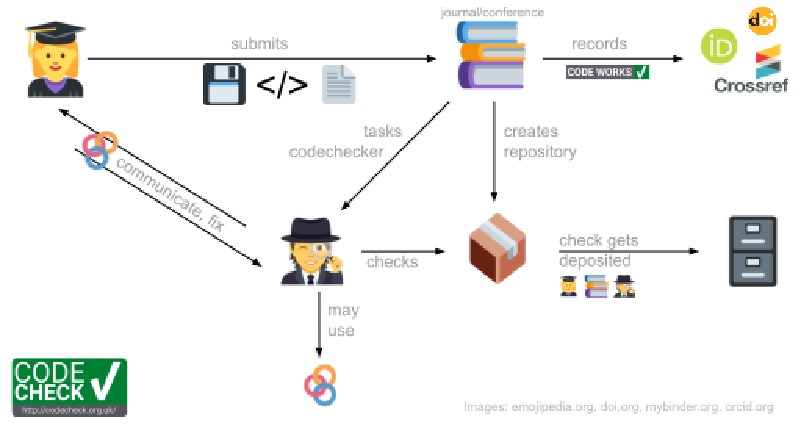
\includegraphics{figs/codecheck_overview.pdf}
  \caption{The detective. Could we number the arrows as steps?
(Implementing the CODECHECK process).  DANIEL: could you check whether
the icons are reusable.}
  \label{fig:worfklow}
\end{figure}

\subsection*{Variations}\label{variations}

DANIEL: COULD YOU DO THIS SECTION ON DIMENSIONS?
This example workflow leaves sufficient room for different
implementations of this process. There are several aspects that can be
considered:

\subsubsection*{When to do a codecheck}\label{when-to-do-a-codecheck}

preprint (no publisher available), pre-condition for peer review, during
peer review, after acceptance. Each of these have their own pros/cons.

\subsubsection*{Who does the codecheck}\label{who-does-the-codecheck}

in house staff, pool of ECRs, volunteeres, for inhouse staff, credit not
an issue.

\subsubsection*{Who knows who?}\label{who-knows-who}

single blind, double blind, private/public communication between author
and codechecker, collaborative. (This might need finessing with
principle 2 below).

\section*{Core principles}\label{core-principles}

The workflow and variations just outlined below reflect our current
views on how a codecheck should be performed. They are not set in
stone, but we do believe the following core principles underpinour
CODECHECK:

\textbf{1. Codecheckers record but don't investigate or fix.} The
codechecker follows the instructions provided by the author in running
the code. If any steps are unclear, or if code does not run correctly,
the codechecker records this fact, and then communicates this
information to the author. We believe that the job of the codechecker is
not to fix all these problems, but simply to report them, and await a
fix from the author.

\textbf{2. Communication between humans is key.} Some code may just work
without any interaction (e.g.~Manuel's certificate); however, more often
there are hidden dependencies that need to be found, or revised software
installations. Allowing the codechecker and human to communicate
directly and openly with each other should make this process as
constructive as possible. We feel that routing this conversation
(possibly anonymously) through a publisher would slow things down and
reduce the chances for community building.

\textbf{3. Credit is given to codecheckers.} (TODO Explain in a few
sentences what each means, e.g.~see 1,2) Ideally publons, or similar,
but can just be a citation to the publicly available DOI. (Community
DOIs use these.)

\textbf{4. Workflows must be auditable.} (TODO Explain in a few
sentences what each means, e.g.~see 1,2)

\textbf{5. Open by default.}  By default, unless there are strong
reasons to the contrary (e.g. clinically-sensitive data), all code and
data, both from author and codechecker, will be made freely available
when the certificate is published, following community principles.


\section*{Register}\label{register}

We have a curated list of 15 certificates available at
\url{https://codecheck.org.uk/register}. These are a mixture of
reproductions of papers for a variety of reasons (do we name them all?)
from interesting historical papers, to papers codechecked as part of
peer review, or because of public interest (covid). several covid models
have been done during the time of peer review of these papers, under our
initative rather than requested from journal, but certificate have then
been acknowledged/cited in the paper (LANCET / LSHTM).
Table~\ref{tab:register} lists the certificates completed to date,
along with citations to the original papers.

The bulk of the certificates fall into three themes: (1) `classic'
papers from computational neuroscience (2) Covid modelling preprints
(3) AGILE.  We would like to briefly highlight three examples here.

\begin{enumerate}
\def\labelenumi{\arabic{enumi}.}
\item
  Gigascience -- our first paper. Only visualisation, not machine
  learning (which would have taken sseveral days of compute time).
\item
  report 9 -- covid model of UK lockdown model -- unlike many claims
  in the popular media at the time, the model was reproducible
  [NOORDEN news piece]. 
\item
  Manuel's certificate -- approached us as he requested a certificate
  as paper was entering peer review.
\end{enumerate}


(DANIEL: say something about the Agile bundle, and the origins?)

\begin{table}
  \centering

  \begin{tabular}{lllp{9cm}} \toprule Certificate & Ref & Research
    area & Description \\ \midrule 2020-001 & \cite{cert-2020-001} &
    Machine learning & CODECHECK undertaken post acceptance of
    manuscript and before its publication in \textit{Gigascience}
    \cite{Piccolo2020-lo}.
    \\
    2020-002 & \cite{cert-2020-002} & neuroscience & Paper from 1997
                                                     showing
                                                     unsupervised
                                                     learning from
                                                     natural images
                                                     \cite{Hancock1992-mp}.
    \\
    2020-003 & \cite{cert-2020-003} & neuroscience &
                                                     Classic paper
                                                     from 1982 on
                                                     models of
                                                     associative
                                                     memory
                                                     \cite{Hopfield1982-mz}.
    (Simulation code was written specifically for this project.)\\
    2020-004 & \cite{cert-2020-004} & area & Barto \\
    2020-005 & \cite{cert-2020-005} & area & Larisch \\
    2020-006 & \cite{cert-2020-006} & area & Detorakis \\
    2020-007 & \cite{cert-2020-007} & area & in progress \\
    2020-008 & \cite{cert-2020-008} & Covid & Modelling of
    interventions on Covid  cases in the UK; checked as preprint (NOW REMOVED XXX)
    and now published \cite{Davies2020-vj} \\
    2020-009 & \cite{cert-2020-009} & Covid &  tracing \\
    2020-010 & \cite{cert-2020-010} & Covid &  report 9 \\
    2020-011 & \cite{cert-2020-011} & Covid & Modelling of Covid
    spread across Europe;  paper was checked when in press (now  published) \cite{Flaxman2020-yb}. \\
    2020-012 & \cite{cert-2020-012} & Covid &   Modelling of Covid spread across the USA; preprint currently review \cite{Unwin2020}. \\
    \\ \bottomrule
  \end{tabular}
  \caption{Register of completed certificates.  An interactive version
  of this is available at \url{http://codecheck.org.uk/register}.  SJE
to complete...}
  \label{tab:register}
\end{table}


\subsection*{Annotated certificate}\label{annotated-certificate}

At the completion of each CODECHECK, a certificate is written that
states which figures and tables from the original article could be
reproduced by the CODECHECKER.  This certificate is made freely
available so that all readers of the article can see which elements
have been reproduced.  The certificate also includes links to the code
and data used by the codechecker, allowing others to build on the
work.  The format of the certificates has evolved slightly during the
project, as we have learnt to automate different aspects of the
certification.  

To demonstrate the typical contents of a certificate, in
Figure~\ref{fig:cert} we have annotated the first four (out of ten)
pages of the certificate 2020-012 \cite{cert-2020-012}.  The reference
article \cite{Unwin2020} describes the modelling COVID-19 across the
USA.
%% TODO - has this been published yet?.  No, not yet... in review...
Figure~\ref{fig:cert}A shows the certificate number, and its DOI,
which points to the certificate as archived on Zenodo.  Our logo is
attached to the certificate to denote successful reproduction.
Figure~\ref{fig:cert}B provides the key metadata about the check --
which paper was checked, and who/when it was checked.  Materials
relating to the codecheck are freely available via the Repository
link.  Figure~\ref{fig:cert}C is a summary of how the codecheck was
performed, and any interesting findings.

Figure~\ref{fig:cert}D (page 2 of the certificate) shows a table that
lists the outputs that were generated from the codecheck (this is
termed the MANIFEST.)  For each output, there is a comment stating
which figure/table it should be compared to in the original paper,
along with the size of the file.  On page 3 of the certificate,
Figure~\ref{fig:cert}E shows some more detailed notes from the
codechecker, in this case indicating what steps were needed to
initialize the environment and run the code.  This particular example
was quite long, taking about 17 hours to run.  Finally, on page 4 of
the certificate, we see the first output that was generated by the
codecheck (Figure~\ref{fig:cert}F).  In this case, the figure matches
figure 4 of REF.  Subsequent pages of the certificate show other
outputs (not shown here).



\begin{figure}
  \centering
  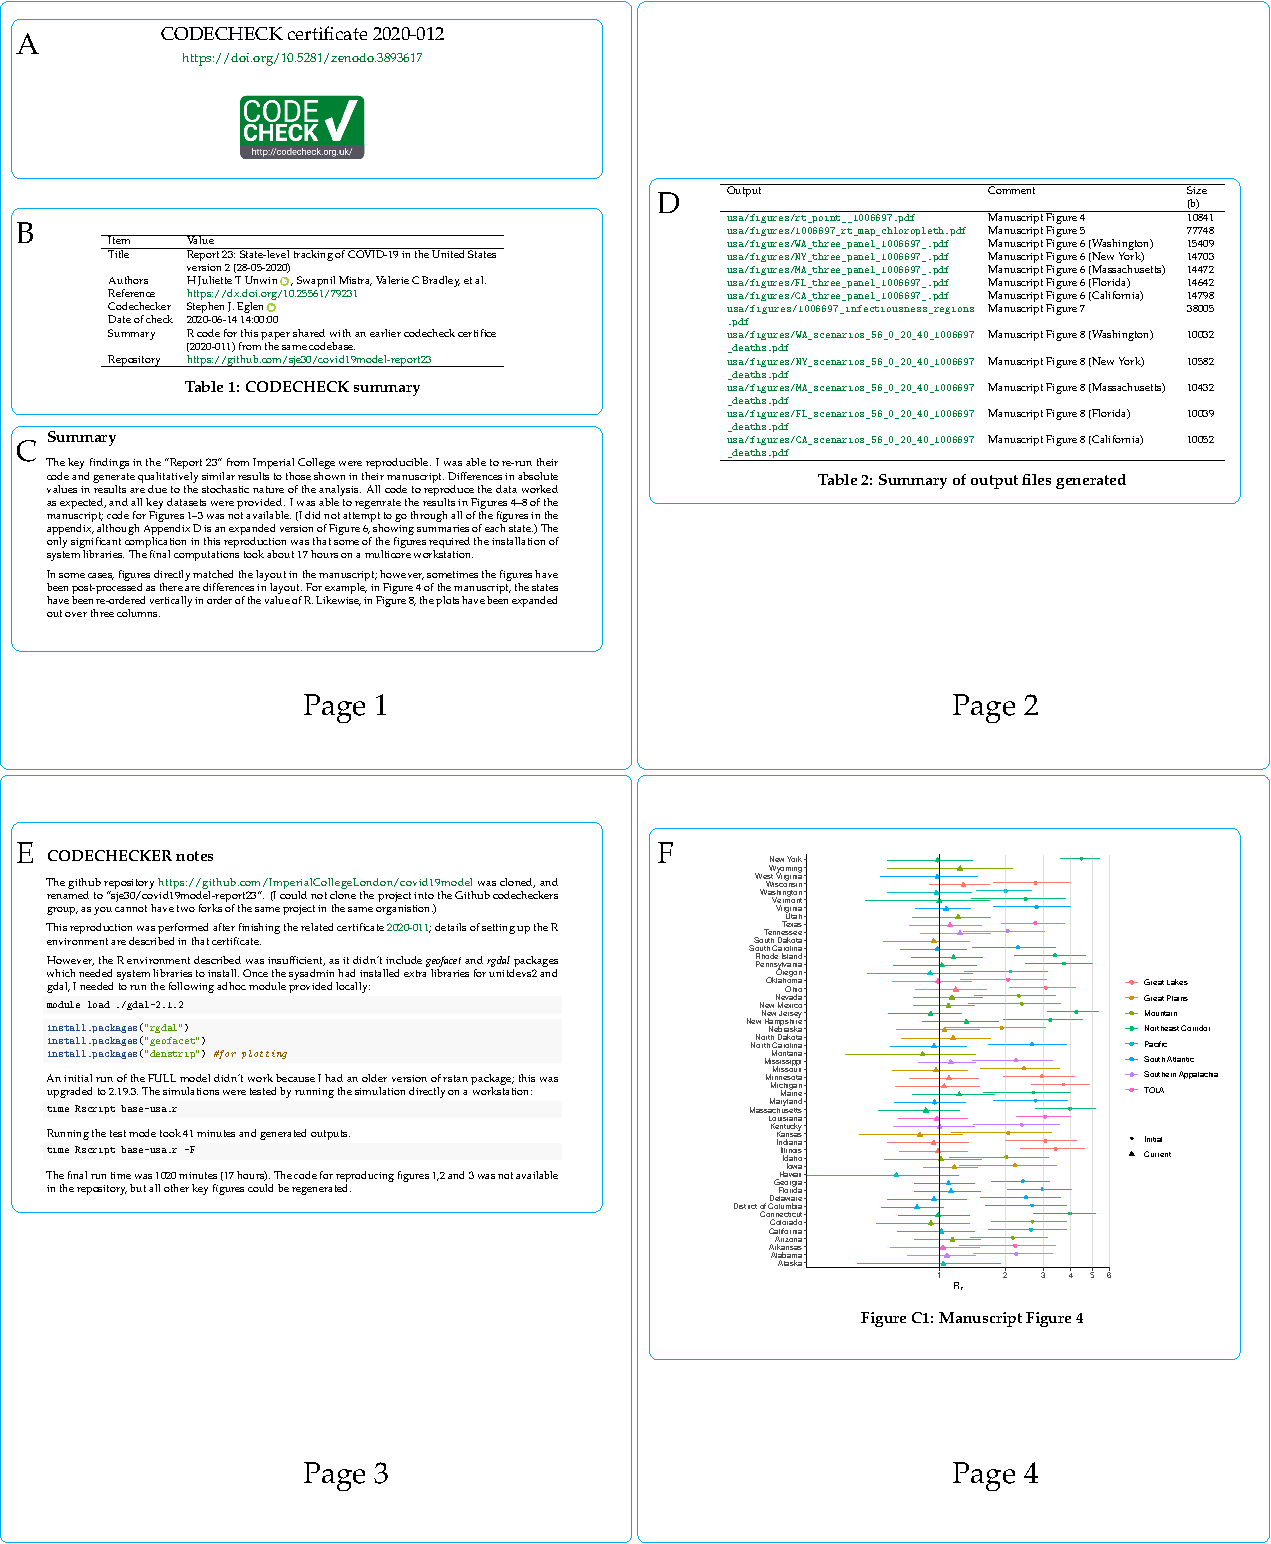
\includegraphics[width=\textwidth]{figs/annotate-cert-crop.pdf}
  \caption{Annotated certificate 2020-012 (first four pages only).}
  \label{fig:cert}
\end{figure}

\subsubsection*{Tools and resources}\label{tools}

To run the system, we rely on github to host our work, and use a
custom R pacakge, codecheck, to help with the generation of
certificates and depositing work on zenodo. (Cite zen4R).  You can do
everything with open infrastructure (e.g.~automated rendering of
register). but you can use your own tools if you prefer.

\section*{Related work}\label{related-work}

TO BE CONTINUED.

All the related projectsfrom A-Z\ldots{} e.g.~CASCAID, Rescience,
modeldb, o2r. Community iniatives like reprohack along similar lines of
checking code. \url{https://reprohack.github.io/reprohack-hq/}

DELIBERATEY NOT COMPREHENSIVE HERE.

\section*{Limitations}\label{limitations}

\textbf{Handling failure}: we have no established process for this, as
so far all our codechecks succeeded. Open question remains as what to do
in this case -- should we publicly report that the code would not run.

\textbf{Compute time}: for those papers that take significant compute
time (think days, not minutes), who will pay for the compute time?

\textbf{Software}: authors can currently provide code that requires
propieratiry software. Given the prevalence of software like MATLAB,
this seems like a pragmatic choice, but then (a) we can't rely on open
infrastructure like mybinder, (b) codechecker must have that software.

\textbf{Can't someone cheat?} yes. we don't check it is correct code,
just simply that it runs. Very low bar. But by having the code open,
interested parties can then examine the code, and knowing that the code
will be open we hope will be an incentive for authors to share.

\textbf{Who's got time for more peer review?} Agree, but ECRS might be
attracted to working with groups (recall it is not anonymous)

\textbf{Who finds the codechecker?} Good point! The journal. Community
however think this is an important issue, and are volunteering.

\textbf{Checking multiple times?}  If you check a preprint before peer
review, it might need checking again as it is modified during peer
review.  Unavoidable, and as happened to us (2020-012 has been
revised).  But checking the manuscript the second time is likely to be
much less work than the first time.

As a principle, we do not require results to be exactly the same for a
codecheck to pass, simply that the code runs and generates the output
files that the author claims. Stochastic simulations mean that often
we cannot get exactly the same, or even different versions of
libraries.  (Cite freesurfer example \cite{Gronenschild2012-pp} that
generates different outputs on different operating systems).

\begin{itemize}
\item modelDB principle: minimum of one figure should be reproducibe.
  Example certificate 2020-016 (I think) which had only a small subset
  of the possible figures. Still useful and worth sharing.
\end{itemize}

\section*{Future work and conclusions}\label{future-work-and-conclusions}

\begin{itemize}
\item
  possibility to allow CI for open papers such that for ``nearly free''
  we can find out when softwave breaks, and if provenance tools are
  used, when.
\item
  How to embed this in journals.
\item
  When is CODECHECK redundant? will it become part of regular peer
  review? or, if ayuthors become more skillful, then everything becomes
  automated, and no need for codecheck. CODECHECK disappearing is then a
  measure of success.
\end{itemize}

Or will it always be adjunct to peer review, and needed?

working within the trad system of publishers to help push the
conversation along.




\subsection*{Competing interests}

SJE is on the senior editorial board at the journal \emph{Scientific
Data}.

\subsection*{Grant information}

This work was financially supported by the UK Software
Sustainability Institute and a Mozilla Science mini grant.

\subsection*{Acknowledgements}\label{acknowledgements}

Collaborators and potential collaborators:

We are grateful to the following individuals for discussions regarding
the work presented here: Andy Collings, Melissa Harrison, Giuliano
Maciocci (eLife), Rebecca Kirk (PLOS Computational Biology), Scott
Edmunds (Gigascience) Andrew Hufton (Scientific Data). Iain Davies and
Yuhao (Sebastian) Wang developed code and example certificates.

\subsection*{Author contributions}

DN and SJE contributed equally to all aspects of this project.


{\small\bibliographystyle{unsrtnat}
\bibliography{bibliography}}




%%%%%%%%%%%%%%%%%%%%%%%%%%%%%%%%%%%%%%%%%%%%%%%%%%%%%%%%%%%%%%%%%%%%%%

\clearpage
\begin{itemize}
\item
  role of data and code, data science
\item
  reproducible resarch
\item
  data enclaves
\item
  CASCAID
\item
  ROpenSci/PyOpenSci (and how their software review differs, though they
  also collaborate with journals,
  \url{https://devguide.ropensci.org/softwarereviewintro.html})
\item
  time capsules \textgreater{}
  \url{https://twitter.com/DougBlank/status/1135904909663068165?s=09}
\item
  science is changing:
  \url{https://theconversation.com/what-you-need-to-know-about-how-coronavirus-is-changing-science-137641}
\item
  reproducibility is important, also

  \begin{itemize}
  \item
    effects on well-being/mental health,
    \url{https://www.nature.com/articles/d41586-020-01642-9}
  \end{itemize}
\end{itemize}

\textbf{main contributions}

\begin{itemize}
\item
  a concept for integrating a minimal code review into common scholarly
  communication processes around peer review
\item
  set of shared principles (recognition value) that allow researchers to
  quickly understand the level of evaluation across
  journals/publishers/conferences, and allows helps these stakeholders
  to establish workflow checking in their domain/solution/product
\item
  a common language and rubric for classifying different levels of code
  and data evaluation as part of a peer-review
\end{itemize}

\section*{What is CODE CHECK?}\label{what-is-code-check}

\begin{itemize}
\item
  \textbf{Principles}: \url{https://codecheck.org.uk/}
\item
  relation to ``proper'' citation of data and software, and depositing
  of data and software in suitable repos \emph{besides} the bundle for
  CODE CHECK: do it, only provide the concrete analysis script for the
  check
\item
  \textbf{Why is it useful?}

  \begin{itemize}
  \item
    reduce the barrier to evaluating non-text parts of research
  \item
    acknowledges different skill sets and existing high load on
    reviewers
  \item
    CC breaks problem that publishers staff expertise today is not
    likely to suffice
  \item
    engaging ECRs is a perfet fit (they are up-to-date in methods, are
    introduced to peer review)
  \item
    relation to research compendia? point it out for authors unsure
    about how to structure their workflow
  \item
    CrossRef and Publons and ORCID have features around reviews
  \item
    shifting burden from reviewer to author (but not too much)
  \item
    What issues with (open) peer review does CODECHECK address?
  \end{itemize}
\item
  keynote \url{https://doi.org/10.7557/5.4963}: in discussion, the
  speaker mentioned value of peer review for ``baseline reassurance'',
  i.e.~a paper has at least been checked by someone with an
  understanding, to increase trust especially if looking at papers from
  other disciplines
\item
  \textbf{report} must fulfil some requirements to make clear what is
  really checked and not mislead - readers will have very different
  understandings of a green checkmark!
\item
  reproducibility is hard
  \url{https://twitter.com/annakrystalli/status/1144176149859377152?ref_src=twsrc\%5Etfw}
  \textgreater{} code check gives at least some benefits
\item
  what are the requirements / level or reproducibility required or
  checked?

  \begin{itemize}
  \item
    \href{https://stodden.net/icerm_report.pdf}{Stodden et al., 2013}:
    five-level hierarchy of research - reviewable, replicable,
    confirmable, auditable, and open or reproducible
  \item
    \href{https://figshare.com/articles/Showing_your_working_A_guide_to_reproducible_neuroimaging_analyses/4244996/2}{Whitaker
    2017}: reproducible, generalisable, replicability, robustnes
  \end{itemize}
\item
  can authors retract their code/data once a CODECHECK has started? In
  the eLife prepreint review, there seems no ``way back'', see
  \url{https://twitter.com/ceptional/status/1271528976763121664?s=09}
\end{itemize}

\section*{Related work}\label{related-work-1}

\begin{itemize}
\item
  CODECHECK vs.~Verification Reports \textgreater{} \textgreater{}
  \url{https://www.sciencedirect.com/science/article/pii/S0010945220301738\#fn3}
\item
  CODECHECK vs.~the ``Artifacts Evaluated - Functional'' badge of the
  ACM, see
  \url{https://www.acm.org/publications/policies/artifact-review-badging}
\item
  Does CODECHECK do internal replication, as defined by
  \url{https://gatesopenresearch.org/articles/4-17/v2} ?
\item
  \url{https://paperpile.com/shared/rVNwBS}
\item
  Are ``Replicated Computations Results (RCR) Report'' a thing?
  apparently so (using ACM terminology)

  \begin{itemize}
  \item
    \url{https://dl.acm.org/doi/10.1145/3185337}
  \item
    \url{http://users.iems.northwestern.edu/~nelsonb/Publications/Nelson_RCRgreenSim.pdf}
  \item
    \url{https://dl.acm.org/doi/epdf/10.1145/3341094}

    \begin{itemize}
    \item
      citation for replicated workflow lists it as ``to appear''
    \end{itemize}
  \item
    getting proper papers for reproductions != CODECHECK approach where
    we want credit as reviewers
  \item
    see also
    \href{https://www.google.com/search?q=\%22Replicated+Computations+Results+\%28RCR\%29+Report+for\%22}{Google
    Search}
  \end{itemize}
\item
  \url{https://medium.com/bits-and-behavior/a-modern-vision-for-peer-review-d5f73f0fae07}
  - work by Amy J. Ko:
  \url{https://faculty.washington.edu/ajko/publications}

  \begin{itemize}
  \item
    is CODE CHECK's process too small, too incremental a change?
  \end{itemize}
\item
  overview of peer review and bibliometrics (if not a reference itself,
  it gives plenty of references):
  \url{http://juser.fz-juelich.de/record/865096/files/Peer\%20Review\%20and\%20Bibliometrics.pdf}
\item
  Open Peer Review \textgreater{}
  \url{https://researchintegrityjournal.biomedcentral.com/articles/10.1186/s41073-019-0063-9}

  \begin{itemize}
  \item
    Are OPR lessons transferable to CODECHECK? Does CODECHECK work
    better with OPR than with (single/double) blind peer review?
  \item
    similarities to their advice: open reports, give credit
  \end{itemize}
\item
  \emph{Successes and struggles with computational reproducibility:
  Lessons from the Fragile Families Challenge} \textgreater{}
  \url{https://osf.io/preprints/socarxiv/g3pdb/}
\item
  community standards for software, cf.~slide 6 in
  \url{https://figshare.com/articles/_/5675104}

  \begin{itemize}
  \item
    ``good enough practice'' is ``get a colleague to try using it'',
    slide 19 in \url{https://figshare.com/articles/_/5675104}
  \end{itemize}
\item
  journals doing code reviews

  \begin{itemize}
  \item
    \emph{``We know of 16 journals that take this valuable step (ie TOP
    Level 3): AEA as already mentioned, plus others in polisci,
    psychology, biostats, and org chem: see Data Rep Policies here
    \url{https://t.co/plOF8j6ADU}''}
    (\url{https://twitter.com/EvoMellor/status/1202692360456589339?s=09});
    see also whole thread!
  \item
    \url{https://medium.com/@NeurIPSConf/call-for-papers-689294418f43}
  \item
    \url{https://www.journals.elsevier.com/information-systems/editorial-board/}
  \item
    SIGMOD Reproducibility Review?
  \item
    Biostatistics ``AER''
    (\url{https://academic.oup.com/biostatistics/article/10/3/405/293660})
  \end{itemize}
\item
  open science platforms/cloud services \textgreater{}
  \url{https://www.nature.com/articles/d41586-019-03366-x}
\item
  live code in articles \textgreater{} o2r, eLife RDS
  \url{https://www.nature.com/articles/d41586-019-00724-7}, \ldots{}
\item
  Artefact Evaluation - \url{https://www.artifact-eval.org/about.html}
\item
  continuous analysis - \url{https://www.nature.com/articles/nbt.3780}
\item
  ``A Universal Identifier for Computational Results'' \textgreater{}
  \url{https://www.sciencedirect.com/science/article/pii/S1877050911001256}
\item
  Discussion about using Docker containers during JOSS reviews
  \textgreater{}
  \url{https://github.com/openjournals/joss/issues/498\#issuecomment-462046912}
\item
  \url{https://scigen.report}, an independent site for registering
  reproductions, via
  \url{https://annakrystalli.me/talks/ro-reprohack.html\#32}

  \begin{itemize}
  \item
    example
    \url{https://scigen.report/reviews/get?doi=10.1063/1.1823034}
  \item
    seems to be closed infrastructure
  \end{itemize}
\item
  new journal \emph{ReScienceX} (about experiments) also seems to have
  an ECR angle, \url{https://www.nature.com/articles/d41586-020-01328-2}
\item
  really interesting work on reproductions in hydrology, with a neat
  survey that reproducers filled out which might be interesting to
  capture from codecheckers, too:
  \url{https://www.nature.com/articles/sdata201930\#Sec9}
\end{itemize}

\section*{CODE CHECK implementation concepts}\label{code-check-implementation-concepts}

\begin{itemize}
\item
  need to get wording straight: process/implementation/workflow (DN:
  suggest to use ``workflow'' for research-analysis workflow)
\item
  \url{https://codecheck.org.uk/process/}
\item
  \emph{dimensions} along which a check can vary
\item
  independent/pre-submission (Peer\_Coding) by author + colleagues
\item
  AGILE
\item
  premier (OA) publisher
\item
  community OA / scholarly society with public peer review
\item
  invited reproducibility paper track,
  cf.~\url{https://www.elsevier.com/journals/information-systems/0306-4379/guide-for-authors}
\item
  on giving credit: public databases

  \begin{itemize}
  \item
    \url{https://www.reviewercredits.com/}
  \item
    Publons
  \item
    ORCID
  \end{itemize}
\item
  compare with existing processes that are publicly documented

  \begin{itemize}
  \item
    AJPS Verification Policy:
    \url{https://ajps.org/ajps-verification-policy/}
  \item
    \ldots{}
  \end{itemize}
\item
  flexible level of detail? a check can be enhanced to (potentially
  semi-automatically) check for good practices

  \begin{itemize}
  \item
    ``A group of us in the ({\textbf{???}}) Software Citation
    Implementation Working Group produced a''Software Citation Checklist
    for Authors" \url{https://t.co/4Noe66FsoX} providing guidelines on
    how to cite software and describing why it is important and what
    software should be cited" via
    \url{https://twitter.com/alegonbel/status/1207664922932453376?s=09})
  \end{itemize}
\item
  focus on ECR as codecheckers

  \begin{itemize}
  \item
    ECR are the one's breaking new ground in schol comm, cf.~the
    percentages of career stages submitting registered reports on slide
    20 \textgreater{} \url{https://osf.io/2vjus/}
  \end{itemize}
\end{itemize}

\section*{Annotated Examples}\label{annotated-examples}

\begin{itemize}
\item
  \textbf{the default implementation}
\item
  critically discuss our/the default implementation vs.~the principles
\item
  HPC example
\item
  if we see the corpus of examles as a scientific dataset, it should be
  published in a citable way (maybe even submit to a data journal)
\end{itemize}

\section*{Open problems}\label{open-problems}

\begin{itemize}
\item
  Do publishers need to build up data science experts who can conduct
  checks?
\item
  Is an integration of software/data citation checks
  benefitial/realistic?
\item
  Bot-support and tools (linter, report authoring with R Markdown)
\item
  How can open platforms be used to enable a review in private
  (cf.~\url{https://www.cambridge.org/core/blog/2019/08/19/how-to-make-the-data-and-code-for-your-manuscript-available-to-peer-reviewers-before-making-it-public/}),
  if that is desired
\item
  Does nudging towards better practices work (highlight the successes)
  or is any check with opt-in doomed to fail?
\item
  Do we need more than one codechecker? Is there a similar diversity as
  in a peer review where more opinions are needed?
\item
  can CODECHECK work for preprints? how? is a re-check required?
\item
  Risk: is the hurdle too low? are ``levels'' of checks are solution to
  increase transparency of check's level of detail
\item
  CODECHECK in the context of innovations and disruptions in scientific
  publishing

  \begin{itemize}
  \item
    \url{https://doi.org/10.1042/ETLS20180172}
  \item
    \url{https://doi.org/10.3390/publications7020034}
  \end{itemize}
\item
  Should every code be checkd, or should the labour be capped by only
  checking ``important'' works or at important stages; if yes, isn't
  peer review such a stage?
\item
  see \url{https://github.com/codecheckers/discussion}
\item
  Can we establish code checks as a type of review within the schol comm
  metadata (or should we?) \textgreater{} we should not, put them on the
  same level as reviews!
\item
  How can we turn a CODECHECK into a positive experience?

  \begin{itemize}
  \item
    cf.~kindness in peer review in
    \url{https://www.mdpi.com/2304-6775/8/2/26}
  \end{itemize}
\item
  How can we allow reactions to checks? (commenting on reports)
\item
  Will bitwise reproducibility become easier than what a CODECHECK does?
  triggered by
  \url{https://twitter.com/khinsen/status/1242842759733665799?s=09})
\item
  If a report is not published for failures: Isn't there a bias for the
  codechecker to have a ``successful'' reproduction because then a
  report is published?
\end{itemize}

\end{document}
